% <- percent signs are used to comment
\documentclass[12pt]{article}

%amsmath is a packaged use for typesetting math
%amsfonts is required for special fonts, e.g. blackboard bold (for denoting real numbers, etc.)
\usepackage{amsmath,amsfonts}

%graphicx is required for images
\usepackage{graphicx}

%used for customzing enumarations
\usepackage{enumerate}

%tikz is the package used for trees
\usepackage{tikz}

\usepackage{algo,fullpage,url,amssymb,epsfig,color,xspace}
\usepackage[pdftitle={CS 240 Assignment 0},%
pdfsubject={University of Waterloo, CS 240, Spring 2016},%
pdfauthor={}]{hyperref}

\renewcommand{\thesubsection}{Problem \arabic{subsection}}

%Note: Many of the packages above have other uses beyond those used in this document

%this marks the beginning of the document. Everything before this is called the Preamble.
\begin{document}
%marks the end of the title section
\begin{center}
{\Large\bf University of Waterloo}\\
\vspace{3mm}
{\Large\bf CS240R \& CS240E, Spring 2016}\\
\vspace{2mm}
{\Large\bf Assignment 0}\\
\vspace{3mm}
\textbf{Due Date: Wednesday, May 11, at 5:00pm}
\end{center}

\definecolor{care}{rgb}{0,0,0}
\def\question#1{\item[\bf #1.]}
\def\part#1{\item[\bf #1)]}
\newcommand{\pc}[1]{\mbox{\textbf{#1}}} % pseudocode

Please read
\url{http://www.student.cs.uwaterloo.ca/~cs240/s16/guidelines.pdf}
for guidelines on submission.  For problems 1 -- 6, submit your
solutions electronically as a PDF file using MarkUs.
This assignment is worth up to 6 bonus marks, which will be added to
your total mark for assignment 1.


%\section marks off a section, adding a * at the end doesn't number the section 
%\section*{Introduction}
A0 is designed to introduce you to \LaTeX{}.
We strongly encourage students to create all their assignment solutions using \LaTeX{},
as it will strongly benefit both you and your markers. Learning \LaTeX{} is a great asset 
to have for any course, and also especially for those of you planning to go into academia.
\LaTeX{}, like HTML, is best learned by example. To complete the problems below, open the 
\LaTeX{} file used to make this PDF. Inside the file you will find the code used to write this
file along with comments explaining the code to help you get through the assignment. If you get
stuck there are also many on-line resources you can use. Searching for ``fraction example \LaTeX{}'' 
is acceptable. Searching for ``\LaTeX{} proof of summation from 1 to n'' 
is {\bf not} acceptable. To compile the .tex file provided simply type ``pdflatex a0.tex" 
in the school's Linux environment. \LaTeX{}  compilers are also free to download on-line.
{\bf Submit both a0.pdf and a0.tex to Markus}.

%\clearpage

\section*{Problem 1 - Assignment Guidelines}
At tht top of this page is the URL to the assignment guidelines for CS240, it can also be found from the course webpage from the Assignments tab. Please answer the following questions about the assignment guidelines:

\begin{enumerate}[a)] 
	\item If an assignment question asks you to design an algorithm, what must you do in addition to describing/writing the pseudocode for the algorithm?
	\item For programming questions, which function can you use to read input? \\ Which functions can you use to output the answer?
\end{enumerate}

\section*{Problem 2 - Mathematics}
In CS 240, you will be using many mathematical concepts. It is important to be able to typeset mathematics in your assignments. This will include sums, fractions, subscripts \& superscripts, etc. \\
Example: 
$$\bar{f}(n) := \sqrt {\sum_{i=0}^{\lg n} 4^i \left ( \frac{n_0}{2^i} \right )^{\theta}}.$$
\\
In order to practice this skill, write a proof showing: $$\sum_{i=1}^n i = \frac {n(n+1)} {2}$$

\section*{Problem 3 - Trees}
CS 240 introduces many tree data structures. Here is a balanced BST on 7 letters of the 
alphabet. Insert the first three letters of your first name into the tree (if your first 
name is shorter than 3 letters, simply insert all the letters), starting 
with the first letter of your name. If you are inserting duplicate
letters:

\begin{enumerate}[a)]
	\item Find the largest index of the letter you are inserting. 
	\item Insert your letter, with an index one larger than the index you found.
	\item When comparing to an equal value, follow the left branch.

\end{enumerate}

For example, if you were to insert a `M' into the tree below, it would be entered as M$_1$ and it would become the right child of I$_0$. Only show the resulting tree.

\begin{center}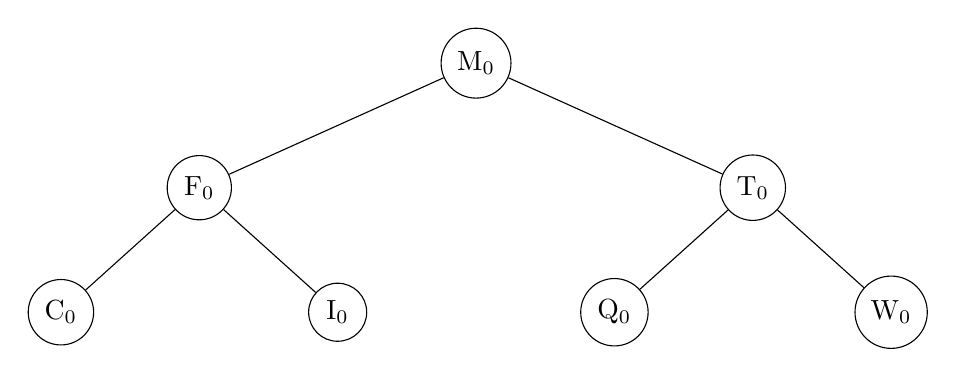
\begin{tikzpicture}[
  level distance=45 pt,
  every node/.style={circle,draw},
  level 1/.style={sibling distance=200 pt},
  level 2/.style={sibling distance=100 pt},
  level 3/.style={sibling distance=60 pt}
]
  \node {M$_0$}
    child {node {F$_0$}
      child {node {C$_0$}}
      child {node {I$_0$}}
    }
    child {node {T$_0$}
      child {node {Q$_0$}}
      child {node {W$_0$}}
    };
\end{tikzpicture}\end{center}

{\it Hint: For nodes with only one child, you may wish to use ``child[missing]'' for the non-existent child.}

%This starts a new page
\clearpage


\section*{Problem 4 - Plots}

CS 240 also deals with many graphs and plots. Plot the following points below, the first one has already been done for you. Only show the resulting plot.\\
Points: (2,7), (7,1), (4,5), (1,3), (3,2), (6,6), (0,9), (9,8), (8,0), (5,4)

\begin{center}
\begin{tikzpicture}
		\draw[thick,]  (0,9) -- (0,0) node[left] {0};
		\draw[thick,]  (0,0) -- (9,0) node[below] {9};
		\draw[thick,]  (9,9) -- (9,0) node[left] {};
		\draw[thick,]  (9,9) -- (0,9) node[left] {9};


		%There are many variations of lines you could draw, you may find the
        %line below helpful in future assignments
		%\draw[thick,dashed,blue]  (5,0) -- (5,9) node[below] {};
		
		\fill (2, 7) circle[radius=2.5pt] node[right]{(2, 7)};

\end{tikzpicture}
\end{center}

\section*{Problem 5 - Tables}
Occasionally, you may want to present information in a table. In \LaTeX{} you can easily
 present data in well structured tables. 
Fill in the table below with any animal you like.\\

 %l stands for left aligned column 
 %c stands for centered column 
 %r stands for right aligned column
 
 % More information on tables http://en.wikibooks.org/wiki/LaTeX/Tables

\begin{tabular}{ | l || r  | r | c | c |} \hline
  Animal's Name & Avg. Weight & Longevity & Avg. Temperature & Conservation Status  \\ \hline
   Polar Bear & 350-700kg & 25 years & 37$^{\circ}$C  & Vulnerable \\ \hline
    & & & & \\ \hline
\end{tabular}

\section*{Problem 6 - Images}
You may find it too time consuming to do parts of your assignment in \LaTeX{}, at which 
point you may want to include an image of your work. \LaTeX{} also supports images. 
Please keep your image sizes small both for this assignment and future assignments; 
however, be sure that your images can be easily read by your markers, or you run the 
risk of losing marks. For this question, include an image of the animal you entered
in the table above.\\


%Note: You do not need to put images in a figure environment.
\begin{figure}
\begin{center}
        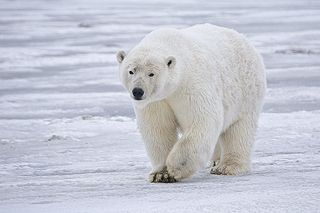
\includegraphics[scale=0.5]{polar_bear.jpg}
\end{center}
\caption{\label{figcaption} Polar bear}
\end{figure}

\end{document}
